\documentclass[12pt,a4paper]{article}
\usepackage{amsmath,amssymb,amsthm,epsf, graphicx, rotating}
\usepackage{fancyhdr}
\usepackage{subfig}
\usepackage{float}
\graphicspath{ {./images/} }

\pagestyle{empty}
\setlength{\parindent}{0pt}
\setlength{\textwidth}{6.5in}
\setlength{\oddsidemargin}{0in}
\addtolength{\textheight}{1in}

\renewcommand\theenumi{\alph{enumi}}
\renewcommand\labelenumi{(\theenumi)}

\newcommand{\Z}{\mathbb{Z}}
\newcommand{\F}{\mathbb{F}}
\newcommand{\R}{\mathbb{R}}
\newcommand{\C}{\mathbb{C}}
\newcommand{\N}{\mathbb{N}}
\renewcommand\vec{\mathbf}

\pagestyle{fancy}
\fancyhf{}
\fancyhead[LE, RO]{Ryan Liu}

\theoremstyle{definition}
\newtheorem{problem}{}

\author{Ryan Liu}
\title{MATH 442 Homework 6}
\begin{document}

\begin{center}
{\huge MATH 442 \par}
{\Large Homework  6  \par}
{\normalsize Name: Ryan Zhuo Lun Liu \par}
{\normalsize Student Number: 30328141 \par}
{\normalsize Collaborators: Robert Benjamin Lang }
\end{center}

\begin{problem} \underline{Answer:}
\begin{proof} This will be proved both ways. \\
For $\rightarrow$ \\
Suppose that $G_1$ and $G_2$ are homeomorphic. Consider $H_1$, the maximal reduction of $G_1$, is obtained by removing vertices of degree 2 until vertices of degree 2 no longer exist in the graph. The same process can be repeated to obtain $H_2$ from $G_2$. \\

Since $G_1$ and $G_2$ are homeomorphic, then $H_2$ can be obtained from $G_1$ and $H_1$ can be obtained from $G_2$. Thus, $H_1$ and $H_2$ must be isomorphic. \\

For $\leftarrow$ \\
Suppose that $H_1$ and $H_2$ are the maximal reductions of $G_1$ and $G_2$ respectively. Consider that $H_1$ is obtained by removing vertices of degree 2 until vertices of degree 2 no longer exist in the graph. Now, since $H_1$ and $H_2$ are isomorphic, $H_2$ can also be obtained from $G_1$ following the same process with some slight modifications. \\

Since $H_2$ is the maximal reduction of $G_2$, then we can reconstruct $G_2$ from $H_2$. As shown above, $H_2$ can be obtained from $G_1$ as well, implying that $G_1$ and $G_2$ are homeomorphic.
\end{proof}
\end{problem}

\begin{problem} \underline{Answer:}
\begin{proof}
The first graph is planar. Figure 1 is a planar drawing of it.

\begin{figure}[H]
    \centering
    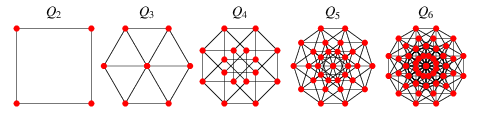
\includegraphics[scale=0.6]{q2.png}
    \caption{Graphs G needed for L(G) to be $K_3$ and $K_4$}
    \label{fig:my_label}
\end{figure}

Unfortunately I could not come up with a subgraph of 2 such that it is homeomorphic to either $K_5$ or $K_{3,3}$.
\end{proof}
\end{problem}

\begin{problem} \underline{Answer:}
\begin{proof}
Suppose that $G_1$ and $G_2$ are homeomorphic.  \\

Consider $H_1$, the maximal reduction of $G_1$, which is homeomorphic to $G_2$, as $G_1$ is homeomorphic to $G_2$. This relationship can be said to be true for $H_2$ as well. Thus, $H_1$ and $H_2$ are isomorphic, meaning that they have the same number of vertices and edges ($m_3$ and $n_3$). \\

Consider the steps to obtain $H_1$. We started from either $G_1$ or $G_2$ and removed vertices of degree 2 until vertices of degree 2 no longer exist in the graph. In this process, the number $m_i - n_i$ would remain unchanged as we lose one vertex and one edge. \\

Thus, if $G_1$ and $G_2$ are homeomorphic, we have $m_1 - n_1 = m_2 - n_2$.
\end{proof}
\end{problem}

\begin{problem} \underline{Answer:}
\begin{proof}
Suppose a graph $G$ is a simple planar graph with 24 edges and 8 faces and each vertex has degree of at least 3.\\

Following Euler's formula that $v - e + f = 2$, we see that with the above configuration, $v = 2 - f + e = 18$. However, given that the graph has exactly 24 edges and that each vertex has degree of at least 3, the $G$ has maximum 8 vertices. Thus, this graph cannot exist.
\end{proof}
\end{problem}

\begin{problem} \underline{Answer:}
\begin{proof}
Suppose that $G$ is a regular graph where each vertex has degree $k > 0$. Therefore, every vertex in $G$ has $k$ edges. \\

As each edge will be connected to two vertices, we have to consider both ends. At the first end of the edge, it will be "meeting" $k - 1$ edges. At the second end of the edge, it will still be "meeting" $k - 1$ edges as $G$ is regular. \\

Thus, each vertex in $L(G)$ should have a degree of $2k - 2$ and therefore is a regular graph with degree $2k - 2$.
\end{proof}
\end{problem}

\begin{problem} \underline{Answer:}
\begin{proof}
Consider a graph $G$, then the edges in $L(G)$ can be described as a pair, $(e_1, e_2)$, which also uniquely describes a vertex in $G$. \\

Consider the $i$th vertex $v_i$, which has degree $d_i$. Then for $v_i$, there are $\binom{d_i}{2}$ edges of $L(G)$. Thus the total number of edges in $L(G)$ is \\

$\sum_{i = 1}^{n} \binom{d_i}{2} = \sum_{i = 1}^{n}\frac{d_i(d_i - 1)}{2}.$
\end{proof}
\end{problem}

\begin{problem} \underline{Answer:}
\begin{proof}
To find a graph $G$ such that $L(G) = K_n$ where $n \geq 3$, we can first observe a few requirements. \\

$L(G)$ would have $n$ vertices, $\frac{n(n - 1)}{2}$ edges, and each vertex is of degree $n - 1$ (regular). This would mean that $G$ has exactly $n$ edges. \\

Consider a graph $G$ with $n + 1$ vertices. We place one vertex in the middle and arrange the other $n$ vertices to surround the central vertex. By doing so, we can connect every other vertex to the central vertex with one edge each, totalling $n$ edges. The resulting graph always has exactly one (central) vertex that has $n$ edges "meeting" and thus $L(G)$ will be $K_n$, where every vertex is connected to every other vertex. \\

\begin{figure}[H]
    \centering
    \includegraphics[scale=0.6]{q7.png}
    \caption{Graphs G needed for L(G) to be $K_3$ and $K_4$}
    \label{fig:my_label}
\end{figure}

\end{proof}
\end{problem}

\end{document}
